%%%%%%%%%
\section{Testing for a new resonance hypothesis}\label{sec:stat}
%%%%%%%%%

The purpose of this analysis is to infer a constraint on the existence of a new resonance decaying into diboson for a set of different signal mass hypotheses.
The comparison between the diboson invariant mass distribution observed in data and the SM background prediction is used to check for the presence of the new resonance.
A hypothesis test is built to decide between a null hypothesis given by the predicted SM background only, against an alternative hypothesis which includes both background as well as the sought after signal.
In principle one can either test the background-only hypothesis and exclude it if there is a large deviation of the data from the SM background prediction,
or test the signal hypothesis and exclude it if there is a large deviation of the data from the expected signal model.
In particular, if no significant deviation from the SM background prediction is observed in data, compatible with the signal hypothesis, an upper limit on 
production cross section of such signal is usually set, up to a certain degree of belief.
%From the statistical analysis of the reconstructed diboson invariant mass, one can infer that there is 95\% confidence level (CL) that the signal $\sigma\times\cal B$ is not larger than some value $?_\mathrm{95\%}$;
%otherwise, if the cross section was above this value, a statistically-significant excess of data would have emerged over the background.
%If the upper limit $?_\mathrm{95\%}$ is as large as the $\sigma\times\cal B$ predicted by some specific theoretical model $?_\mathrm{th}$ or smaller, it can be inferred that a resonance of that mass is excluded at 95\% C.L..
The CMS community has agreed upon a procedure for computing upper limits, which is based on the modified frequentist method, often referred to as $\mathrm{CL}_s$.
While a detailed description of such method can be found in Refs.~\cite{CLs1,Junk:1999kv}, the basic ingredients will be summarized Section~\ref{subsec:CLs}.
A description of the procedure followed to quantify an excess of events is provided in Section~\ref{subsec:pvalue}. A summary of the final results will be given in the next chapter.

\subsection{Limit setting procedure}~\label{subsec:CLs}

The procedure to establish the exclusion of a given signal hypothesis is based on a frequentist significance test which uses a log-likelihood ratio as a test statistic.
In order to construct the test statistic a likelihood function is defined as

\begin{equation}\label{eqn:likelihood}
{\cal L}( data | \mu,\theta) = \mathrm{Poisson}(data | \mu\cdot s(\theta) + b(\theta))\cdot p(\tilde{\theta}|\theta).
\end{equation}

In this definition, $s$ and $b$ denote the expected signal and background event yields, respectively,
which, before the scrutiny of the observed data entering the statistical analysis, are subject to multiple uncertainties that are treated by introducing nuisance parameters $\theta$,
so that signal and background expectations depend on these parameters as $s(\theta)$ and $b(\theta)$.
The exclusion of a signal hypothesis is generally expressed as an upper limit on the \textit{signal strength modifier} $\mu$
which scales the cross section used as input in the evaluation of the expected signal yields.
With this definition, the likelihood represents the Poisson probability of observing a certain amount of data when the expected yield is $\mu\cdot s(\theta) + b(\theta)$
and given the probability $p(\tilde{\theta}|\theta)$ of measuring a value $\tilde{\theta}$ for the nominal nuisance parameter $\theta$.
Note that, in this likelihood definition, ``data'' stands for a generic dataset, either experimental or a pseudo-data generated randomly.

The likelihood can be either binned or unbinned. In the first case the function $\mathrm{Poisson}(data | \mu\cdot s + b)$ in Eq.~\ref{eqn:likelihood} is the product of Poisson probabilities
for observing $n_i$ events in each bin $i$ of the signal+background model

\begin{equation}\label{eqn:binned}
\prod_i \frac{(\mu s_{i} +b_{i})^{n_i}}{n_i!}e^{-(\mu s_i + b_i)}.
\end{equation}

For the unbinned case each event enters the calculation as follows

\begin{equation}\label{eqn:unbinned}
k^{-1}\prod_i (\mu S f_s(x_i) + Bf_b(x_i))e^{-(\mu S + B)},
\end{equation}

where $f_s(x)$ and $f_b(x)$ are the probability density functions of signal and background of the observable $x$, while S and B are the total event rates expected for signal and background.
In this analysis the unbinned form for the likelihood is used, where the observable $x$ coincides with the reconstructed diboson invariant mass.\\

To compare the compatibility of the data with the background-only and signal+background hypotheses, where the prediction for the signal is allowed to be scaled by some factor $\mu$,
the test statistic $\tilde{q}_\mu$ is constructed based on the profile likelihood ratio as

\begin{equation}\label{eqn:testStatistic}
\tilde{q}_\mu = -2\ln\frac{{\cal L}(data | \mu,\hat{\theta}_\mu)}{{\cal L}( data | \hat{\mu},\hat{\theta})},\qquad \mathrm{with} \qquad 0 \leq \hat{\mu} \leq \mu.
\end{equation}

Here $\hat{\theta}_\mu$ denotes the value of $\theta$ that maximizes the likelihood for the hypothesized $\mu$,
i.e. it is the conditional maximum-likelihood (ML) estimator of $\theta$ (and thus is a function of $\mu$). 
The procedure of refitting the nuisance parameters to maximize the likelihood for each possible value of the parameter of interest $\mu$, is usually referred to as ``profiling''.
The denominator is the maximized (unconditional) likelihood function, i.e., $\hat{\mu}$ and $\hat{\theta}$ are the global maximum of the likelihood.
The presence of the nuisance parameters broadens the profile likelihood as a function of $\mu$ relative to what one would have if their values were fixed.
This reflects the loss of information about $\mu$ due to the systematic uncertainties.
Higher values of $\tilde{q}_\mu$ correspond to increasing incompatibility between the data and the hypothesized signal of strength $\mu$.
The lower constraint for $\hat{\mu}$ in the denominator excludes the possibility of negative signal yields. 
The upper constraint is introduced to avoid that data with $\hat{\mu} > \mu$ (upward fluctuations) are considered as representing less compatibility with $\mu$ than what obtained with data.

The observed value of the test statistic, $\tilde{q}_\mu^\mathrm{obs}$ for the given signal strength modifier $\mu$ under test is computed,
as well as the nuisance parameters $\hat{\theta}_0^\mathrm{obs}$ and $\hat{\theta}_\mu^\mathrm{obs}$ maximizing the likelihood under the background-only and signal+background hypothesis, respectively.
Furthermore, the probability density functions of the chosen test statistic $\tilde{q}_\mu$ under the signal+background hypothesis, $f(\tilde{q}_\mu|\mu,\hat{\theta}_\mu^\mathrm{obs})$,
and the background-only hypothesis, and $f(\tilde{q}_\mu|0,\hat{\theta}_0^\mathrm{obs})$, are constructed by means of ensembles of toy MC pseudo-experiments
generated according to the same Poisson probabilities used to build the likelihood. In this process the nuisance parameters 
are fixed to the values $\hat{\theta}_0^\mathrm{obs}$ and $\hat{\theta}_\mu^\mathrm{obs}$ obtained by fitting the observed data.

Using the $f(\tilde{q}_\mu|0,\hat{\theta}_0^\mathrm{obs})$ and $f(\tilde{q}_\mu|\mu,\hat{\theta}_\mu^\mathrm{obs})$ distributions,
two p-values are computed

\begin{equation}
\begin{gathered}
p_\mu \equiv \mathrm{CL}_{s+b} = P(\tilde{q}_\mu \geq \tilde{q}_\mu^\mathrm{obs}|\mu s(\hat{\theta}_\mu^\mathrm{obs}) + b(\hat{\theta}_\mu^\mathrm{obs})) = \int_{\tilde{q}_\mu^\mathrm{obs}}^{+\infty} f(\tilde{q}_\mu|\mu,\hat{\theta}_\mu^\mathrm{obs})d\tilde{q}_\mu \\
p_0 \equiv \mathrm{CL}_{b} = P(\tilde{q}_\mu \geq \tilde{q}_\mu^\mathrm{obs}|b(\hat{\theta}_0^\mathrm{obs})) = \int_{\tilde{q}_\mu^\mathrm{obs}}^{+\infty} f(\tilde{q}_\mu|0,\hat{\theta}_0^\mathrm{obs})d\tilde{q}_\mu.
\end{gathered}
\label{eqn:pvalues}
\end{equation}

The two probabilities are shown in the example in Fig.~\ref{fig:CLs-ex_a}.
In the classical frequentist approach, the level of agreement between the data and hypothesized $\mu$ is evaluated by using the $\mathrm{CL}_{s+b}$ probability only,
and one says that the hypothesized signal $\mu$ is excluded at 95\% CL if $\mathrm{CL}_{s+b} \leq 0.05$.

However, such a definition as a caveat. If the distributions of the test statistic for the signal+background and background-only hypotheses have a not negligible overlap as in the plot (c) of Fig.~\ref{fig:CLs-ex_b},
the experiment would tend to exclude the hypothesized signal $\mu$ even if the experiment in this case has little sensitivity to discriminate it against the background.
In fact, in this case the experimental data are highly contaminated with background and a statement about the signal would be a mistake of interpretation.
To prevent the inference of a signal in such cases, the so-called modified frequentist approach has been introduced at the time of LEP~\cite{CLs1,Junk:1999kv}.
In this approach, the level of agreement between the data and hypothesized $\mu$ is evaluated by using instead the quantity 

\begin{equation}
\mathrm{CL}_s = \frac{\mathrm{CL}_{s+b}}{\mathrm{CL}_b},
\end{equation}

and the hypothesized signal $\mu$ is excluded at 95\% confidence level (CL) if $\mathrm{CL}_s \leq 0.05$.
It is straightforward to see from plot (a) of Fig.~\ref{fig:CLs-ex_b} that, if the distribution of the test statistic for the signal+background hypothesis
is well separated from the background-only distribution, then $\mathrm{CL}_s \sim \mathrm{CL}_{s+b}$ and there is no risk of misinterpretation.

In order to quote, as conventionally done, 95\% CL observed upper limits, the full procedure is iterated for different values of $\mu$, until $\mathrm{CL}_s = 0.05$ is found.
This value of $\mu$ is denoted as $\mu_{95\%}$, and one can infer that the hypothesized resonance X$\rightarrow$WV/VH with a cross section $\mu$-times larger than the one predicted 
by some specific theoretical model $\sigma_{th}$ used as input to the statistical analysis, is excluded at 95\% CL.
In this analysis, model-independent limits on the cross section are set by rescaling the $\mu^{95\%} = \sigma_{95\%}/\sigma_{th}$ by the input cross section in order to obtain $\sigma_{95\%}$.

\begin{figure}[!htb]
\centering
\subfigure[]{\label{fig:CLs-ex_a}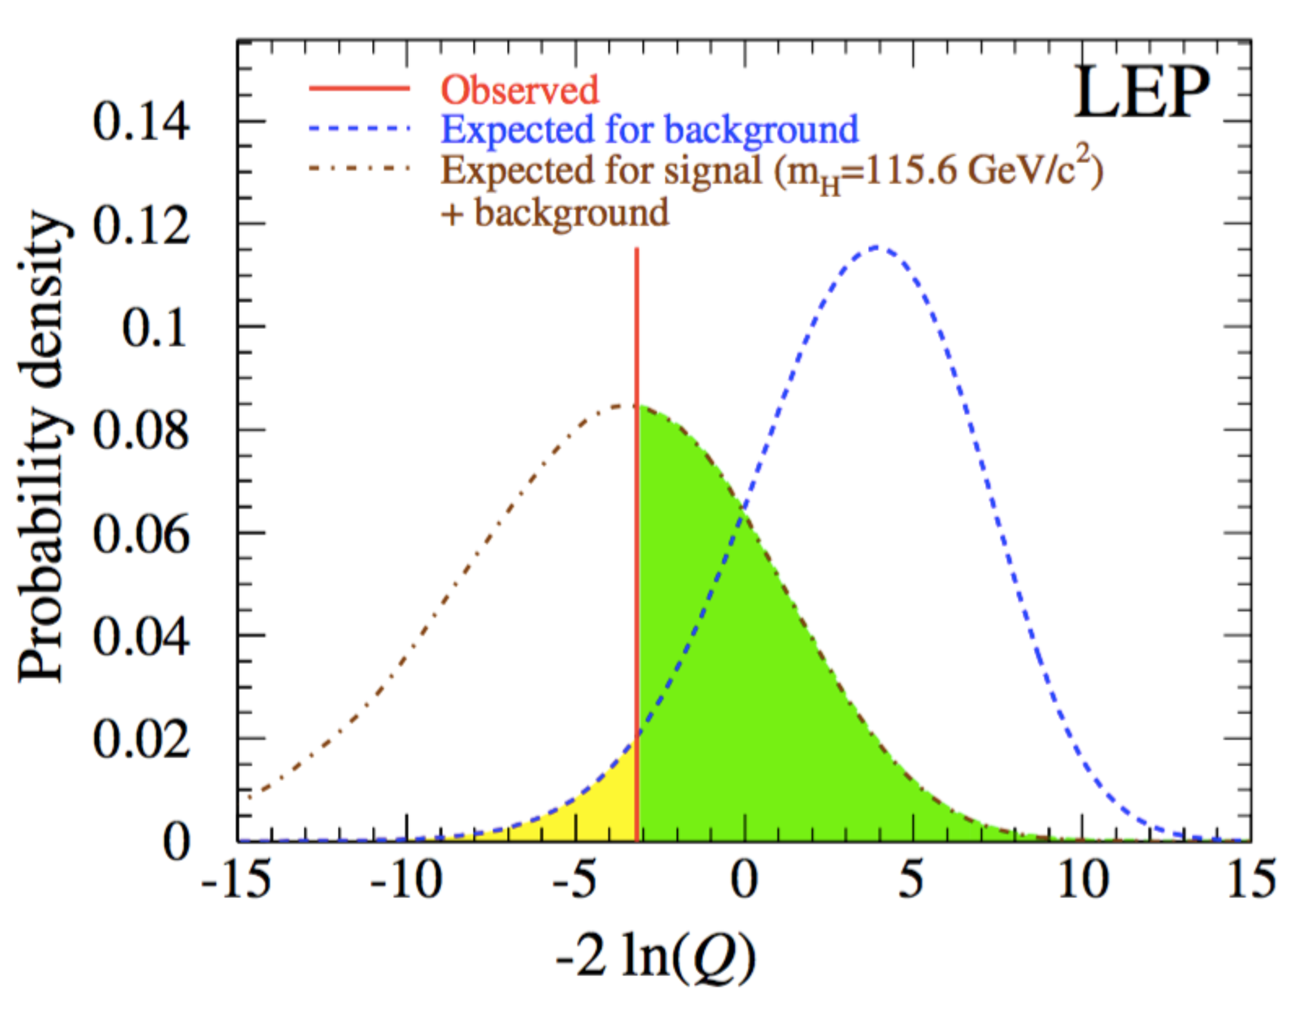
\includegraphics[width=0.55\textwidth]{\cheight/CLs_fig1.pdf}}
\subfigure[]{\label{fig:CLs-ex_b}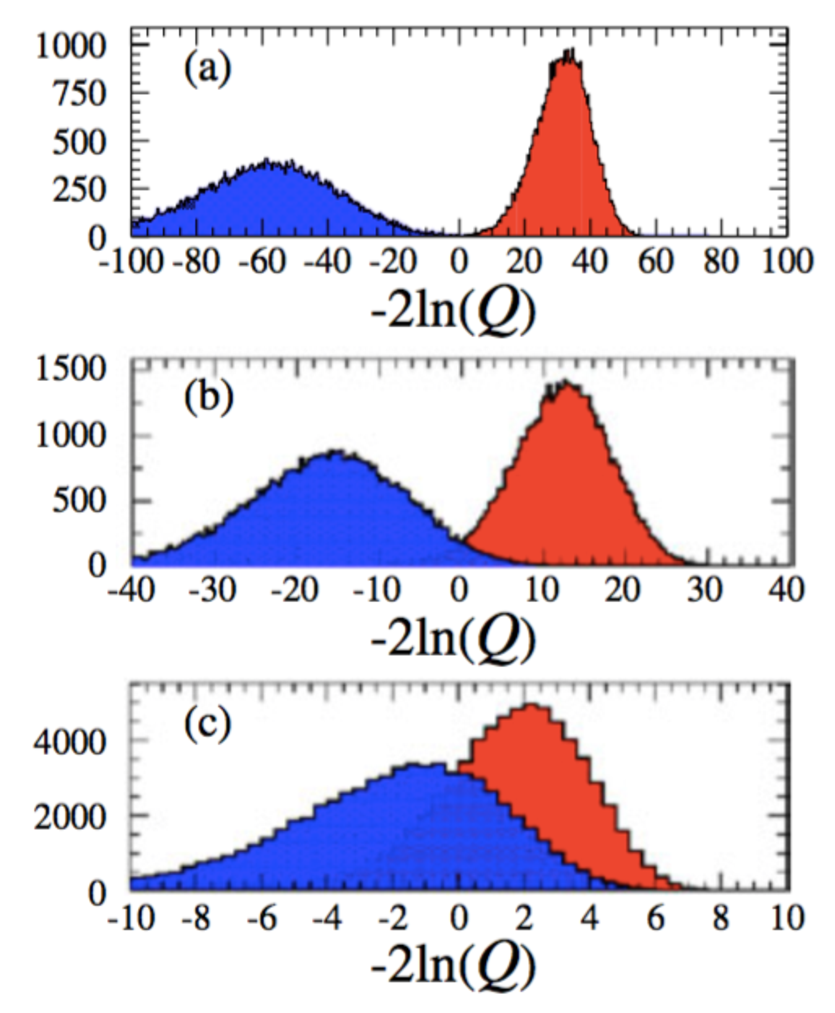
\includegraphics[width=0.35\textwidth]{\cheight/CLs_fig2.pdf}}
\caption{blabla}
\label{fig:CLs-ex}
\end{figure}

In addition to the observed upper limit derived from the actual data distribution, it is important to study also the expected limit given the observed data.
In fact, the expected limit quantifies the sensitivity of the experiment independent from statistical fluctuations in the data.
%The expected $\mathrm{CL}_s$ is extracted by computing the p-values of Equation~\ref{eqn:pvalues} using the median of the 
%$f(\tilde{q}_\mu|0,\hat{\theta}_0^\mathrm{obs})$ distribution instead of the observed value of the test statistic $\tilde{q}_\mu^\mathrm{obs}$.
%In this way a limit is extracted under the assumption that the data lies at the center of the expectation for the background-only hypothesis.
%In addition to the expected limit one can also extract the variation of the expected limit within the uncertainties.
%By using the values of the 16\% (2.5\%) and 84\% (97.7\%) quantiles of the $f(\tilde{q}_\mu|0,\hat{\theta}_0^\mathrm{obs})$,
%instead of the median, the $\pm 1(2)\sigma$ uncertainty bands are obtained.
In order to compute the median-expected upper limit, and the associated $\pm 1\sigma$ and $\pm 2\sigma$ bands,
a large set of background-only pseudo-experiments is generated and, for each of them, the $\mu_{95\%}$ is calculated.
From the cumulative distribution of $\mu_{95\%}$, the median value is taken as the expected limit, while the $\pm 1(2)\sigma$ uncertainty bands on the expected limits
are extracted from the values of the 16\% (2.5\%) and 84\% (97.5\%) quantiles.

\subsection{The asymptotic approximation}\label{subsec:AsymptCLs}

In order to compute the $\mathrm{CL}_s$ the probability density functions of the test statistics are required.
In particular, one needs the probability density functions $f(\tilde{q}_\mu|\mu^\prime)$, where $\mu^\prime = 0$ or $\mu^\prime = \mu$,
which are obtained from MC toys requiring very expensive computational resources.
An approximation for the $\mathrm{CL}_s$ method, valid in the large sample limit, also referred to as ``asymptotic approximation'' has been proposed in Ref.~\cite{AsymptCLs}
and it is briefly described in the following.\\

By using the Wald approximation~\cite{10.2307/1990256} the desired distribution $f(\tilde{q}_\mu|\mu^\prime)$ can be obtained by expressing the test statistic given by the log-likelihood ratio as

\begin{equation}
\tilde{q}_\mu = \frac{(\mu-\hat{\mu})^2}{\sigma^2} + \mathcal{O}(1/\sqrt{N}),
\end{equation}

where $\hat{\mu}$ follows a Gaussian distribution with a mean $\mu^\prime$ and standard deviation $\sigma$, and $N$ represents the data sample size.
For large data samples ($N\rightarrow\infty$), the $\mathcal{O}(1/\sqrt{N})$ can be neglected and it can be shown~\cite{wilks1938} that the distribution $f(\tilde{q}_\mu|\mu^\prime)$ of the test statistic $\tilde{q}_\mu$
follows a \textit{noncentral chi-square} distribution for one degree of freedom with noncentrality parameter

\begin{equation}
\Lambda = \frac{(\mu-\mu^\prime)^2}{\sigma^2}.
\end{equation}

For the special case $\mu^\prime = \mu$ one has $\Lambda = 0$ and the test statistic is distributed as a chi-square for one degree of freedom.
For the general case in which $\mu^\prime \neq \mu$, the standard deviation $\sigma$ of $\hat{\mu}$ has to be evaluated, which depends on the MLE estimator of the nominal nuisance parameters.
The evaluation of $\sigma$ is greatly simplified considering a special, artificial data set, referred to as the ``Asimov data set'', where all statistical fluctuations are suppressed and the estimators for all parameters
are replaced by their expectation values as follows:

\begin{equation}
\hat{\mu} = \mu^\prime \qquad\qquad \mathrm{and} \qquad\qquad \hat{\theta} = \theta.
\end{equation}

With these assumptions the test statistic $\tilde{q}_{\mu,A}$ for the Asimov dataset is given by 

\begin{equation}
\tilde{q}_{\mu,A} \approx \frac{(\mu-\mu^\prime)^2}{\sigma^2} = \Lambda.
\end{equation}

From the Asimov data set one therefore obtains an estimate of the noncentrality parameter $\Lambda$ that characterizes the distribution $f(\tilde{q}_\mu|\mu^\prime)$.
Equivalently, the above equation can be used to obtain the variance $\sigma^2$ which characterizes the distribution of $\hat{\mu}$, namely,

\begin{equation}
\sigma_A^2 = \frac{(\mu-\mu^\prime)^2}{\tilde{q}_{\mu,A}},
\end{equation}

so that the distribution obtained by using $\sigma_A^2$ has a median given by the corresponding Asimov value $\tilde{q}_{\mu,A}$. 
Using these formulae, asymptotic relations are derived which are easily solved for the observed upper limits with the $\mathrm{CL}_s$ method,
as well as for the expected median and error bands.

\subsection{Quantifying an excess of events}~\label{subsec:pvalue}

The presence of the signal is quantified by the background-only p-value, i.e. the probability for the background to fluctuate
and give an excess of events as large or larger than the observed one.
As for the upper limits, this evaluation requires defining a test statistic and the construction of its probability density function.
For a given resonance mass hypothesis $M_X$, the test statistic used in this case is $\tilde{q}_0$, defined as

\begin{equation}
\tilde{q}_0 = -2\ln\frac{{\cal L}(data | 0,\hat{\theta}_0)}{{\cal L}( data | \hat{\mu},\hat{\theta})},\qquad \mathrm{with} \qquad \hat{\mu} \geq 0.
\end{equation}

%The constraint $\hat{\mu} \geq 0$ gives an accumulation of the test statistic at zero for events with downward fluctuations, since we are not interested in interpreting a deficit of events with respect to the expected background on an equal footing with an excess.
The probability density function $f(\tilde{q}_0|0,\hat{\theta}_0^{obs})$ is built by generating toy MC pseudo-data under the assumption of the background-only hypothesis.
From this distribution, the p-value corresponding to a given experimental observation $q_0^{obs}$ is evaluated:

\begin{equation}
p_0 = P(\tilde{q}_0 \geq \tilde{q}_0^\mathrm{obs}|b(\hat{\theta}_0^\mathrm{obs})) = \int_{\tilde{q}_0^\mathrm{obs}}^{+\infty} f(\tilde{q}_0|0,\hat{\theta}_0^\mathrm{obs})d\tilde{q}_0.
\end{equation}

This probability is converted into a \textit{significance}, also referred to as \textit{Z value}, as follows

\begin{equation}
Z = \Phi^{-1} (1-p_0).
\end{equation}

A significance of 5$\sigma$, corresponding to a p-value of 2.87$\times$10$^{-7}$, is conventionally used in high energy physics to claim a discovery,
and 3$\sigma$ for an evidence.

It can be demonstrated that in the asymptotic approximation (Section~\ref{subsec:AsymptCLs}), the likelihood ratio test statistic $\tilde{q}_0$
follows a chi-square distribution for one degree of freedom, and a fair estimate of the p-value and of the significance can be obtained from the observed value $\tilde{q}_0^\mathrm{obs}$ itself,
without the need for generating pseudo-data, as follows

\begin{equation}
\begin{gathered}
p_0 = \frac{1}{2} [ 1 - \mathrm{erf}(\sqrt{\tilde{q}_0^\mathrm{obs}/2}) ] \\
Z = \sqrt{\tilde{q}_0^\mathrm{obs}}.
\end{gathered}
\end{equation}

%\sqrt{\tilde{q}_0^\mathrm{obs}/2}
The p-value discussed above is evaluated at a fixed resonance mass $M_X$ and can be referred to as a \textit{local p-value}.
In this search, a scan is performed over a wide range of resonance mass hypotheses with the aim of finding
the minimum local p-value, which describes the probability of a background fluctuation for that particular resonance mass hypothesis.
However, it is important to distinguish the probability of finding a fluctuation in some particular location from the probability of finding such a fluctuation anywhere else.
The former is associated to the so called \textit{local significance}, whereas the latter is referred to as the \textit{global significance}.
The fact that the global significance is usually smaller than the largest local one is often referred to as the ``look-elsewhere effect'' (LEE).
As demonstrated in Ref.~\cite{Gross:2010qma}, the global and local p-values are related to each other by a multiplicative factor, usually referred to as ``trial factor'', proportional to the number of independent search regions.
In the asymptotic approximation the trial factor grows linearly with the local significance, through a proportional constant
that is related to the ratio between the mass range under consideration divided by its resolution. In particular, it can be shown that

\begin{equation}\label{eqn:trials}
trial\# = \frac{p_{global}}{p_{local}} \approx \frac{1}{3}\frac{mass\ range}{mass\ resolution}Z_{local}.
\end{equation}

The trial factor is best estimated through MC methods as it will be shown in Section~\ref{sec:signif8TeV}. However, a good agreement with the equation above is obtained.